\section{$\frac{1}{2}$-Approximation}
To restate the problem, we are given a graph $G$, vertices $a,b$ and an edge budget $k$. In the decision variant of this problem, we are given a target ratio of $\tau$, but generally we would like to make the ratio of $a$ and $b$'s closeness centrality in the augmented graph as close to 1 as possible. \\\\
Observe that if $a$ and $b$ are ever connected, the worst possible ratio is $\frac{1}{2}$. This happens when every vertex other than $a,b$ in the graph is directly connected to $b$, and $a$'s only neighbor is $b$ itself (see Figure). For large $n$, $b$'s closeness centrality is $1$ times $n$ vertices, while $a$'s is $2$ times $n$ vertices, giving us closeness ratio of $\frac{1}{2}$. If $a$ was closer than $b$ to any vertex, then the numerator would increase and denominator would decrease, giving us a better ratio. Similarly, if any vertex was further than distance 1 from $b$, we would get a better ratio (think $\frac{2}{3},\frac{3}{4}$, etc.). In short, with $a$ and $b$ connected, we guarantee a closeness ratio at least $\frac{1}{2}$.
\begin{figure}
    \centering
    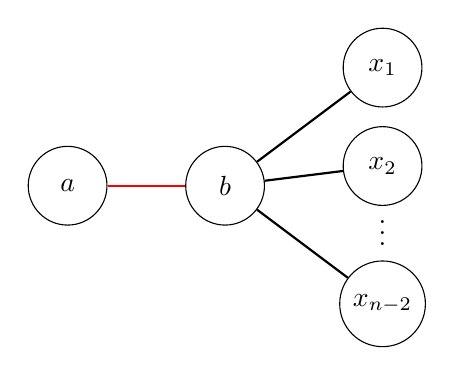
\begin{tikzpicture}[
        node/.style={circle, draw=black, minimum size=1cm},
        edge/.style={thick, -}
    ]
    
    % Define nodes
    \node[node] (A) at (0, 0) {$a$};
    \node[node] (B) at (2, 0) {$b$};
    
    % Draw edge between A and B
    \draw[edge, thick, red] (A) -- (B);
    
    % Define and connect nodes X_1 to X_n
    \node[node] (X1) at (4, 1.5) {$x_1$};
    \node[node] (X2) at (4, 0.25) {$x_2$};
    \node at (4, -0.5) {$\vdots$}; % Dots to represent continuation
    \node[node] (Xn) at (4, -1.5) {$x_{n-2}$};
    
    % Connect B to each X node
    \draw[edge] (B) -- (X1);
    \draw[edge] (B) -- (X2);
    \draw[edge] (B) -- (Xn);
    
    \end{tikzpicture}
    \caption{Worst case of closeness ratio when $a$ and $b$ are connected.}\label{2-apx}
\end{figure}\\\\
Now consider the algorithm, given $k\geq 1$ edges, which simply adds the edge $ab$ (if it does not already exist in the graph). As we just argued, our closeness ratio is now at least $\frac{1}{2}$ (though it might be better). This agrees very well with our hardness results, as we showed getting a target ratio greater than $\frac{1}{2}$ in all cases is NP-hard, but getting a target ratio of exactly $\frac{1}{2}$ is easy (in fact, it only requires one edge). \\\\
Furthermore, this strategy is a $\frac{1}{2}$-approximation for CRI. Whatever ratio an optimal efficient algorithm (which we do not know how to find, as this problem is NP-hard) would achieve on an instance of CRI, our algorithm will never get a ratio less than half of that value. This follows from the observation that, simply by our definition of closeness ratio, a ratio better than 1 is not possible. Thus is we guarantee a ratio of $\frac{1}{2}$, we guarantee that our algorithm produces no worse than $\frac{1}{2}$ of the optimal ratio. \\\\
An important distinction in this section is the difference between \textit{target} ratio and \textit{approximation} ratio. The approximation ratio is the ratio of the closeness ratio our algorithm achieves over the closeness ratio achieved by an optimal algorithm. Connecting $ab$ immediately achieves a target ratio of $\frac{1}{2}$, and as the best possible closeness ratio achievable is $1$, this strategy necessarily forms \textit{at least} at $\frac{1}{2}$ approximation. However, it is possible that this strategy is in fact better than a $\frac{1}{2}$-approximation. That is, all the problem instances where this strategy gets a ratio of $\frac{1}{2}$, an optimal strategy actually cannot get a ratio of 1 (meaning then the ratio of our ratio over optimal ratio is greater than $\frac{1}{2}$).\\\\
TIGHTNESS OF 1/2 EXAMPLE.